\documentclass[11pt, a4paper,twocolumn]{jarticle}
\usepackage[dvipdfmx]{graphicx}
\usepackage{listings,jlisting}

\begin{document}
%=============================================================
\section{受光回路の作成}
\subsection{目的}
走査計測に必要となる受光回路を作成する.
また,今回作成する受光回路は最終日まで使用する.
\subsection{手順}
半田ごてを用いて図に示すように受光回路の作成を行った.
この時受光回路のプリント基板を金属の作業台にそのまま置いてショートさせないように注意した.

\begin{figure}[ht]
 \begin{center}
  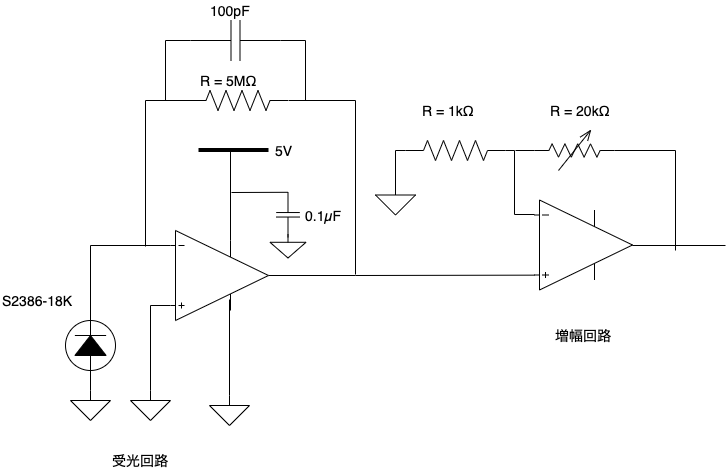
\includegraphics[width=0.8\linewidth]{fig1.png}
 \end{center}
 \caption{受光回路}
 \label{fig:1}
\end{figure}

\subsection{結果}
フォトダイオードに蛍光灯の光を入射させ,手で覆い隠す操作を繰り返しオシロスコープで出力電圧を確認したところ手で覆い隠すと出力電圧は0付近になり,手をどけると60Hz付近の周波数の出力波が観測された.
また可変抵抗${R_2}$を調節することで受光回路の感度を調節できることを確認できた.

\subsection{考察}
手で覆うことで出力が0付近になり,手をどかすことで出力電圧を観測できたことから受光回路は正常に機能していると考えられる.
また手をどかした際に60Hz付近の出力電圧を観測したのは蛍光灯などの教室内の電化製品から発せられる電磁波が観測されたためであると考えられる.
これは西日本の交流電流の周波数が60Hzであることに一致する.
%=============================================================
\newpage
\end{document}
